\section{基于P2P网络的信息自主流动机制的研究}
本章将基于上一章提出的用户兴趣模型给出建立用户兴趣覆盖网络的基本思路和方法。首先,从宏观上给出整个网络的组织架构和拓扑结构,由于是非中心化的P2P,因此网络中的每个节点既要充当服务端也可以作为客户端,如何能够快速发现兴趣相同的节点在信息传播中是尤为重要的。然后,从微观上来看,每个节点存储的信息是决定整个网络流动是否顺畅的基础,因此本章将充分利用用户兴趣集的特性来构建节点存储结构,并阐述如何利用该结构快速找到潜在的目标节点。

\subsection{用户兴趣覆盖网络的构建}
在第二章中提到了用户之间遵循一种关注-被关注的关系,这在社交网络中是十分常见的,因此这里直接将这种关系引入,默认用户节点直接会实现存储一些时常关注的邻居节点。整个网络的架构如图\ref{fig:overlay}所示,图(A)是节点初步连接后的结果。可以看到,在用户关注关系层上,用户$u_1$和用户$u_3$并没有直接的关注或被关注的关系,$u_3$必须先后间接通过$u_4$和$u_3$才能连接到。但是在上面的用户兴趣关系层中,用户$u_1$和$u_3$之间直接建立了关系,依据是他们拥有共同的兴趣(图中绿色边表示)。此时,用户$u_1$充当的是服务器,他将自己的资源1和资源2分别传播给了另外三个用户,并且转播的依据是存在共同兴趣。当经过一系列运作以后,用户兴趣关系层中的拓扑结构会发生变化,如图(B)所示。可以看到,用户$u_4$和$u_1$、$u_2$之间发现了新的兴趣(图中蓝色边表示)。此时,用户$u_4$作为信息发布者将资源3传播给这两个节点,因此$u_1$此时充当了资源接受者,但同时$u_1$也在继续发布资源1,它充当了两个角色。这就是基于P2P网络的一个实例,在构建这样一个覆盖网络归结起来要解决这样两个问题:
\begin{itemize}
  \item 节点的数据存储结构:因为整个网络是一个非结构化的拓扑,也就是说没有中心服务器来直接获得其他节点的信息。所以,每个节点必须自己存储其他部分节点的信息。
  \item 节点间兴趣导向边的建立:节点与节点之间的关系在用户兴趣关系层上表现为两个用户具有共同的兴趣。以上一章的用户兴趣模型来看,也就等价于两者的兴趣集中存在公共兴趣点集合。
\end{itemize}

\begin{figure}[ht]
\centering
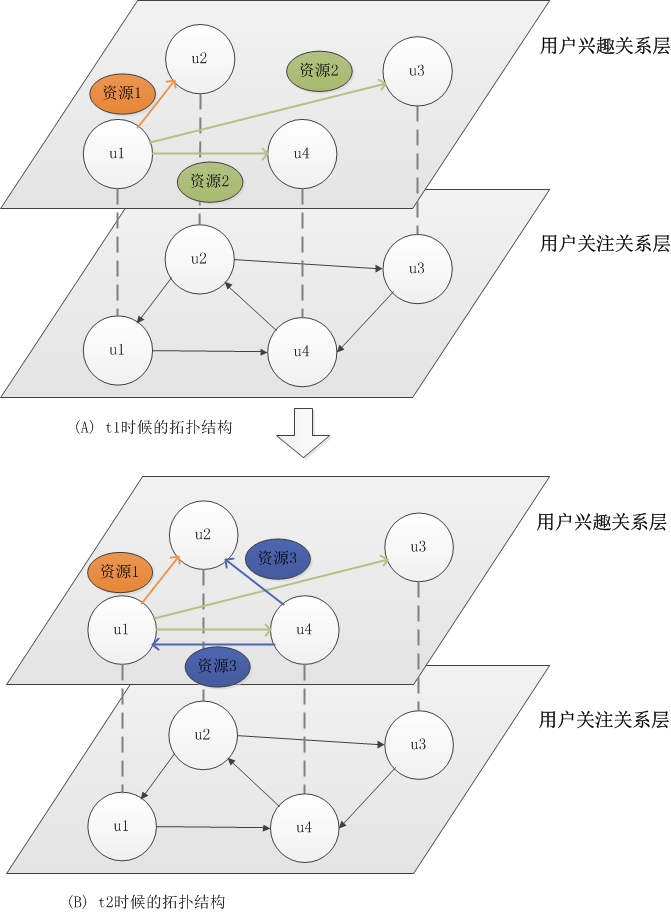
\includegraphics[width=\textwidth]{overlay.png}
\caption{基于P2P的兴趣覆盖网络示意图}
\label{fig:overlay}
\end{figure}

\subsubsection{节点的数据存储结构}
在基于P2P的兴趣覆盖网络中,几乎所有节点都会既要充当信息发布者,又要充当信息接受者,既同时作为服务器和客户端。考虑到这种网络的特性,需要给节点加入以下一些松耦合的规则才能形成。虽然最终得到的拓扑结构具有一定属性,但数据项的设计不能像结构化拓扑中的那样基于任何拓扑相关的知识。先要找到一个数据项,对等查询其邻居,最典型的查询方法是泛洪。查找查询协议充斥于所有的邻居在一定范围内。这样的设计是非常有弹性的,特别是对于那些进入和离开该系统的节点。然而,目前的搜索机制是不可扩展,并生成在网络上意外负载。

\subsection{兴趣覆盖网络拓扑结构的更新}
//todo

\subsection{兴趣覆盖网络的资源传播}
//todo

\subsection{小结}
//todo
